% !TeX encoding=utf8
% !TeX spellcheck=de-DE
% !TeX root=../UID_Project_Documentation.tex

\section{Iteration}

Die bereits im Kapitel \enquote{User Test} diskutierten Verbesserungsmaßnahmen wurden erwartungsgemäß umgesetzt.
Zusätzlich haben wir aber noch von uns aus einige Anpassungen vorgenommen, welche auch in Bezug auf die Vorlesungseinheit \enquote{Mobile UX} aufkamen.

Da der Nutzer auf einem mobilen Gerät aller Wahrscheinlichkeit nach mehrere Apps nebenbei geöffnet hat und er somit auch sehr stark abgelenkt ist, ist es wichtig, dass er zu jedem Zeitpunkt, an dem er wieder zu unserer App zurückwechselt, genau weiß, wo er sich befindet. Um dieses \enquote{Design for interrupts}-Paradigma zu berücksichtigen, haben wir uns dazu entschlossen, in der Action Bar jedem Screen einen entsprechenden Titel zu geben. Wenn man also beispielsweise einen Feed erstellt, und eine Zeitung ausgewählt hat, sodass man nun die Kategorien auswählen muss, steht in der Action Bar der Titel der Zeitung, für welche man die Kategorien auswählt.

\begin{wrapfigure}{R}{0.45\textwidth}
  \centering
  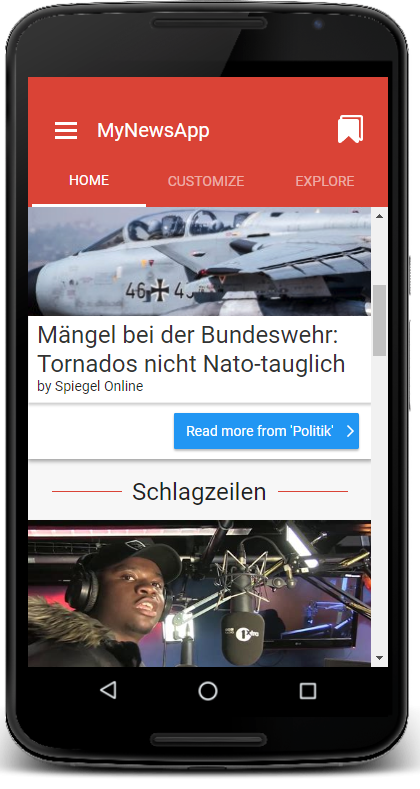
\includegraphics[width=0.4\textwidth]{screenshot 01}
  \caption{\enquote{Home} Ansicht der MyNewsApp}
  \label{fig:screenshot-01}
\end{wrapfigure}

Um mehr Übersichtlichkeit auf dem Homescreen zu schaffen, haben wir eine besser erkennbare Untertrennung der einzelnen Feeds umgesetzt. Feedüberschriften sind vom Rest des Textes abgesetzt und durch minimale Farbwechsel des Hintergrunds bei jedem Feed kann man auch bei schnellem Scrollen schnell erkennen wo die Feeds beginnen und aufhören. Die Buttons, die dafür zuständig sind, mehr von einem Feed anzuzeigen, sind ebenso auffälliger.

Um die gespeicherten Inhalte schneller zu erreichen, wurde der \enquote{Saved Articles}-Feed durch eine Bookmarks-Seite ersetzt. Diese lässt sich leicht durch das Lesezeichen-Piktogramm in der Menüleiste des Homescreens erreichen.

\clearpage

\begin{wrapfigure}{L}{0.45\textwidth}
  \centering
  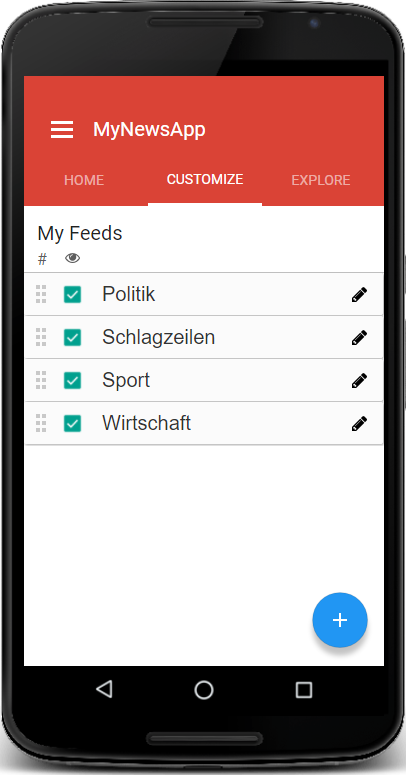
\includegraphics[width=0.4\textwidth]{screenshot 02}
  \caption{\enquote{Customize} Ansicht der MyNewsApp}
  \label{fig:screenshot-02}
\end{wrapfigure}

Die größten Änderungen hat der Menüpunkt Customize erfahren. Man erhält eine Übersicht aller Feeds, mit der Möglichkeit diese für den Homescreen anzupassen. Jeder Listeneintrag ist per Drag-and-Drop verschiebbar und kann unsichtbar geschalten werden. Durch kleine Piktogramme in der Kopfzeile der Liste werden diese Funktionen erklärt. Drückt man auf den Stift, so wird man direkt in die Bearbeitung des Feeds geschickt. Dabei ändert sich der Titel in der Menüleiste entsprechend um anzuzeigen, wo sich der Benutzer gerade befindet, falls nicht sicher ist wo genau er gedrückt hat oder falls er nach App-switchen nicht mehr genau weiß wo er war.

\clearpage

\begin{wrapfigure}{R}{0.45\textwidth}
  \centering
  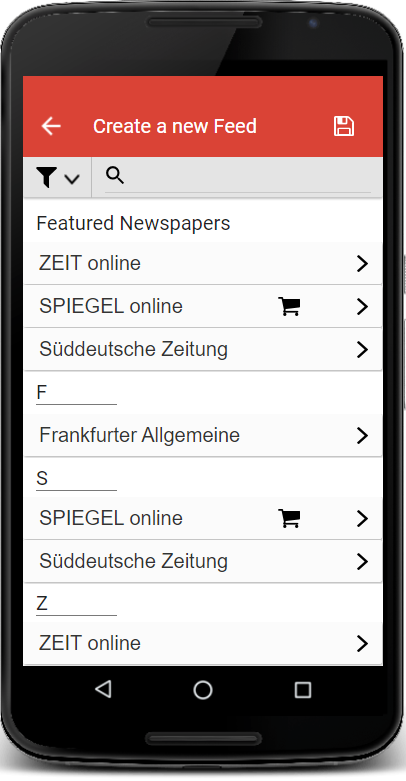
\includegraphics[width=0.4\textwidth]{screenshot 03}
  \caption{\enquote{Create a Feed} Ansicht der MyNewsApp}
  \label{fig:screenshot-03}
\end{wrapfigure}

Bei der Überarbeitung des Menüs zur Erstellung neuer Feeds wurde ein starker Fokus darauf gelegt, die Erstauswahl übersichtlicher zu gestalten. Auf dem Screen sieht man jetzt im ersten Schritt nur eine Auswahl aller verfügbaren Nachrichtenquellen in alphabetischer Reihenfolge. Eine kurze Featured-Sektion hilft dem Benutzer bei der Auswahl. Durch eine Suche und einen Filter für Kategorien lässt sich die Auswahl einschränken. Ist eine Auswahl getroffen, können im zweiten Schritt die Kategorien per Checkbox ausgewählt werden. Um nicht die Übersicht über ausgewählte Nachrichtenquellen zu verlieren, wird bei dem entsprechenden Titel im Obermenü ein Haken gesetzt, sobald man eine Kategorie in dieser Nachrichtenquelle ausgewählt hat. Um den Feed zu speichern, haben wir ein Disketten-Piktogramm, an dem für Android typischen Ort, eingeführt.

\clearpage

\begin{wrapfigure}{L}{0.45\textwidth}
  \centering
  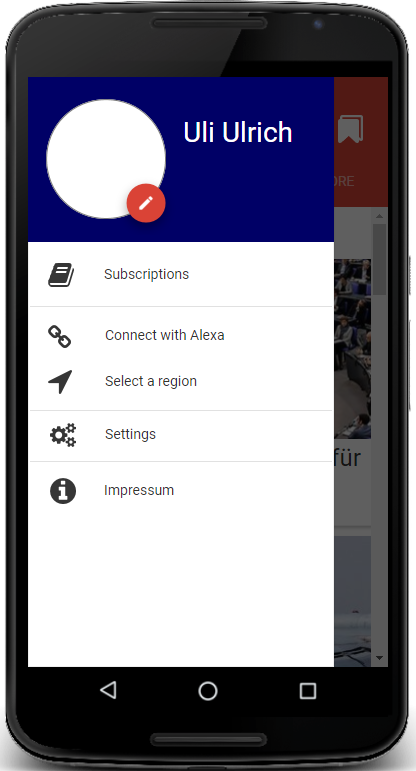
\includegraphics[width=0.4\textwidth]{screenshot 04}
  \caption{\enquote{User} Ansicht der MyNewsApp}
  \label{fig:screenshot-04}
\end{wrapfigure}

In das Burgermenü haben wir, um auch die neuesten Technologien einzubinden, die Option \enquote{Connect with Alexa} hinzugefügt. Digitale Assistenten werden erlangen zunehmend an Bedeutung, wie auch Beliebtheit, sodass dies nicht versäumt werden sollte. Denkbar wäre zum Beispiel, sich Nachrichten vorlesen zu lassen. Natürlich konnten wir die Funktionalität an sich nicht implementieren, aber mit dem Eintrag im Burgermenü sollte gezeigt werden, dass wir auch daran gedacht haben.

Aufgrund der Tatsache, dass wir bei unserer App keine Formulare oder ähnliche Inputs haben, war es nicht nötig, sich Gedanken über sinnvolle Default-Werte zu machen. Dies wäre aber auf jeden Fall zu beachten gewesen, hätte man zum Beispiel eine Registrierungsseite gehabt, bei der man das Herkunftsland auswählen muss. Beim Regionenfilter für Feeds ist es hingegen sinnvoll, den Standort des Nutzers per GPS zu bestimmen und so die Region vor- auszuwählen. Aber auch hier waren uns Grenzen durch Axure gesetzt, sodass wir dies nur durch entsprechende Schaltflächen andeuten konnten.

Im Menüpunkt Explore wurde, analog zu den neuen Piktogrammen in der Menüleiste von anderen Screens, der gewünschte zusätzliche Button zum Hinzufügen von Inhalten implementiert. Dieser ändert sich bei zahlungspflichtigen Inhalten, um ein Einkaufswagen-Piktogramm anzuzeigen. Zahlungspflichtige Inhalte sind außerdem beim Durchstöbern direkt im Titel durch ein Geldschein-Piktogramm erkennbar.

Beim Login wollten wir beachten, dass dieser einerseits schnell gehen muss, andererseits aber auch die typischen Loginmöglichkeiten über zum Beispiel einen Google-Account ermöglicht. Wir haben uns dazu entschieden, dass eine implizite Verbindung mit dem Google-Account hergestellt werden würde, wir also keinen Login-Screen implementieren. Einkäufe laufen dann einfach über das für den Benutzer bekannte System von In-App-Käufen. Würde man die App aber tatsächlich veröffentlichen, sollte man dem Nutzer dennoch die Wahl lassen, wie er sich einloggen möchte.

\clearpage

\begin{wrapfigure}{L}{0.45\textwidth}
  \centering
  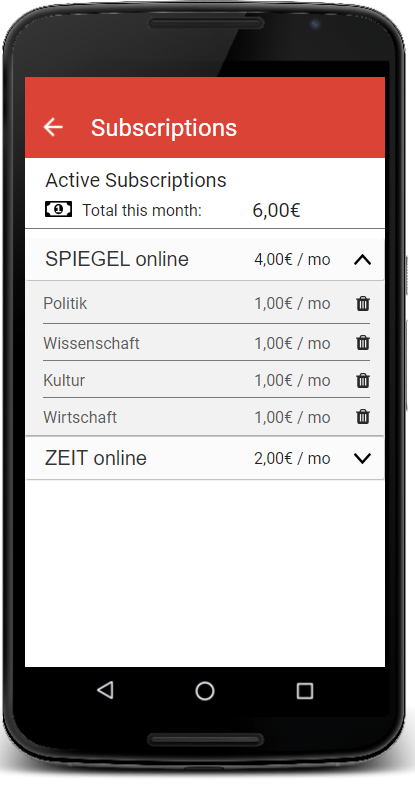
\includegraphics[width=0.4\textwidth]{screenshot 05}
  \caption{\enquote{Subscriptions} Ansicht der MyNewsApp}
  \label{fig:screenshot-05}
\end{wrapfigure}

Eine Möglichkeit zur Personalisierung eines Nutzerprofils darf jedoch in einer modernen App nicht fehlen, wurde aber nur angedeutet, da dies für die App kaum wirklichen Nutzen bietet.

Um Abonnements zu verwalten, haben wir einen komplett neuen Screen entworfen. Eine ausklappbare Liste aller aktiven Abonnements soll mehr Übersicht schaffen. Am Anfang der Liste erhält der Benutzer direkt die Summe für die nächste Abrechnung angezeigt. Dies wird dann zuerst per Nachrichtenquelle und dann noch per abonnierten Inhalt runtergebrochen. Mit dem Mülleimer-Piktogramm kann man den Eintrag direkt löschen. Da dies ohne zusätzliche Abfrage schnell zu Fehlern führen könnte, lässt sich diese Aktion mit Hilfe der Undo-Funktion sofort rückgängig machen. Diese Undo-Funktionalität wurde auch an anderen entscheidenden Stellen (z.b. beim Kauf von neuen Inhalten) eingebaut.
